\chapter{Background}
\label{sec:Background}

\section{Open MPI}
\label{sec:openmpi}
The Open MPI Project is an open source implementtion of the Message Passing Interface (MPI). Open MPI is developed by a consortium of academic, research, and industry partners to combine the expertise, technologies, and resources from the High Performance Computing community and build this MPI library.

Some of the Open MPI features are~\cite{openmpi}:
\begin{itemize}
  \item Open source license
  \item Full conformance with MPI-3 standard
  \item Spawning processes dynamically
  \item Concurrency and thread safety
  \item Support for network heterogeneity
  \item Fault tolerance for network and processes
  \item Support for various job schedulers
  \item Support for all networks in a single library
  \item Portablity and maintainablity
  \item Run-time instrumentation
  \item Support for different operating systems (32 and 64 bit)
  \item Production quality software
  \item Tunable by installers and end-users
  \item Modular component architecture
  \item Documentation for APIs
\end{itemize}
    
\subsection{The Architectire of Open MPI}
Open MPI is built based on a component architecture called the Modular Component Architecture (MCA). Component based archtirecture makes large software projects extensible and maintainable~\cite{barrett2005analysis,graham2006open}. It also allows users to build their own costumized components and integrate them into Open MPI. Component based architectures are popular in the high performance computing community~\cite{squyres2003component,bernholdt2006component}.

Open MPI is comprised of three main functional areas (Figure \ref{fig:MCA_framework})~\cite{graham2006open}:

\begin{figure}[ht]
\centering

\includegraphics[scale=0.4]{images/MCA_framework.png}
\caption[MCA, component frameworks, and the components]{MCA, component frameworks, and the components}
\label{fig:MCA_framework}
\end{figure}

\begin{enumerate}
\item \textbf {MCA}\\
  The backbone modular component architecture that provides management services for all other layers.
  
  The MCA is responsible for management of the component frameworks and providing them services they use. For instance, the MCA provides the ability to accept run time parameters from higher level abstractions (e.g., mpirun) and pass them down through the component framework to individual components. It also finds components at build time and invokes their corresponding hooks for configuration, building, and installation.
  
\item \textbf{Component frameworks}\\
  Each major functional area in Open MPI has a corresponding back end component framework, which manages modules.
  
  Each component framework is a construct that is created for a single, targeted task. For example, \textbf{btl} (Byte Transfer Layer) framework is used to send and receive data on different types of networks, \textbf{allocator} framework is responsible for memory allocation, and \textbf{coll} framework is dedicated to MPI collective algorithms. A framework uses MCA's services to discover, load, use, and unload components at run time. Each framework has different policies and use cases; some only use one component at a time while others use all available components simultaneously.

\item \textbf {Components}\\
  Components are self contained software units that can configure, build, and install themselves. A component is an implementation of a framework's interface. Components are also known as ``plugins''. Each instance of a component is called a ``module''. 

  The Open MPI software has three classes of components: Open MPI (OMPI) components, Open Runtime Environment (ORTE) components, and Open Portable Access Layer (OPAL) components. (Figure \ref{fig:open-mpi-layers})

  Frameworks, components, and modules can be either dynamic or static. This means, they can be available as plugins or they can be compiled statically into libraries.
\end{enumerate}

\begin{figure}[ht]
\centering
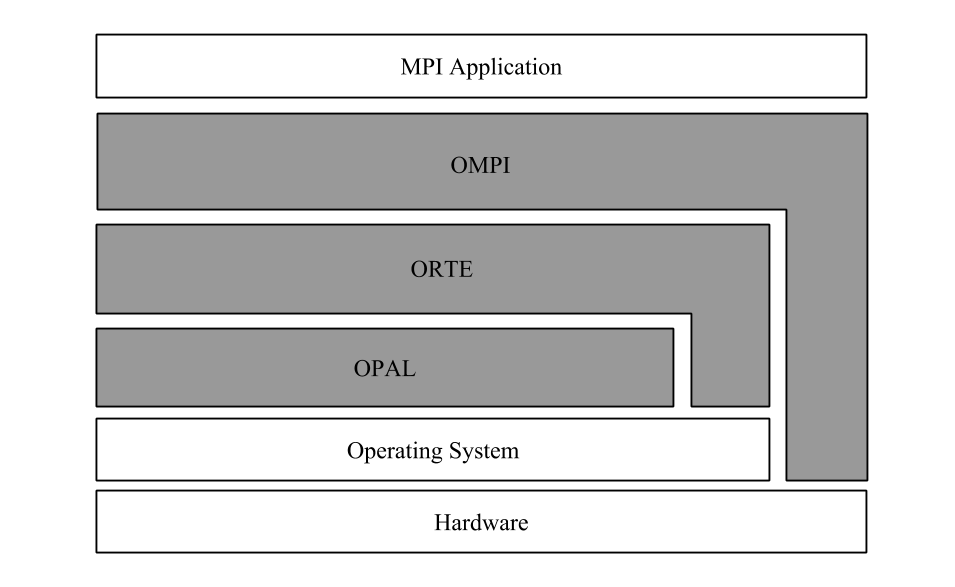
\includegraphics[scale=0.45]{images/open-mpi-layers.png}
\caption{Open MPI Layers}
\label{fig:open-mpi-layers}
\end{figure}


\section{Open Runtime Environment (ORTE)}
\label{sec:orte}
Developing software environments for high performance computing applications in heterogenous distributed systems poses a significant challenge. The runtime environment (RTE) must be capable of supporting heterogeneous operations, efficiently scaling from one to large numbers of processors, and providing effective strategies for dealing with fault scenarios that are expected as our systems continue to scale to exaflop systems~\cite{kronstadt2005peta}.

There has been a number of studies with different approaches to this challenge. Each approach focuses on a particular aspect of the overall problem. For example, LAM/MPI emphasis was on ease of portability and performance~\cite{squyres2004component}. LA-MPI focused on data fault tolerance~\cite{aulwes2004architecture}, and HARNESS FT-MPI focused on system fault tolerance~\cite{fagg2002harness}.

The major roles of every runtime are~\cite{bosilca2011scalability}:
\begin{enumerate}
\item \textbf{Launch}\\
  This task to launch the processes for an MPI application. This is shared between the runtime and the parallel scheduling/launching mechanism.
\item \textbf{Connect}\\
  The connection information (the URI of a process) may not be known before the MPI processes are launched. Therefore, it is necessary for the runtime to establish the connections between the processes.  It is then necessary to distribute this information through an out of band messaging system. 
\item \textbf{Control}\\
  The control role is to ensure that the entire environment is gracefully cleaned in case of a crash. Depending on the operating system and implementation, control may also forward signals to the MPI processes and ensure that completion codes
are returned to the user command: mpirun.
\item \textbf{IO}\\
  The input/output commands launched do not necessarily run on the same machine as where they are issued in an MPI application . However, users usually expect the information printed on the standard output appear on the standard output of the command they launched.  Therefore, it is necessary to forward the standard input/output information to the machine users launch their application from. 
\end{enumerate}

The Open Runtime Environment (ORTE) was developed as a part of the Open MPI project to support distributed high performance computing applications operating in a heterogeneous environment. Implementation of the ORTE is based on the Modular Component Architecture (MCA). The main design objectives of the ORTE are ease of use, resilient operations, scalability, and extensibility. Interprocess communication, resource discovery and allocation, and process launch across different platforms in a transparet manner are main features of the ORTE\cite{castain2005open,hpcwire}.

The ORTE consists of four major subsystems (Figure \ref{fig:orte-architecture})\cite{castain2005open,castain2008open,Castain2008153}:

\begin{figure}[ht]
\centering

\includegraphics[scale=0.43]{images/orte.png}
\caption[The ORTE architecture]{The ORTE architecture}
\label{fig:orte-architecture}
\end{figure}

\begin{enumerate}
\item \textbf{General Purpose Registry (GPR)}\\
  The GPR is the core subsystem in the ORTE architecture. It provides a mechanism for exchanging of communication connection data, in the form of key-value pairs, among processes.  The GPR is also used to synchronize events across the system. It asynchronously notifies subscribers of events such as data changes in the registry or new data being entered to the registry.
\item \textbf{Resource Management}\\
  The resource management subsystem consists of four smaller subsystems: \textit{Resource Discovery Subsytem (RDS)}, \textit{Resource Allocation Subsystem (RAS)}, \textit{Resource Mapping Subsystem}, and \textit{Process Launch Subsystem (PLS)}. These four subsystems together provide services for resource discovery, allocation, mapping, and process launch. 
\item \textbf{Error Management}\\
  The \textit{State Monitoring and Reporting (SMR)} subsystem and the \textit{Error Manager} subsystem are two smaller subsystems constructing the error management subsystem. The error management subsystem brings the fault tolerance capability to the ORTE.
\item \textbf{Support Services}\\
  There are four subsystems comprising the support services subsystem: The \textit{Runtime Messaging Layer (RML)} is responsible for providing administrative communication services across all ORTE subsystems. The \textit{Name Services (NS)} subsystem assigns each application, and each process within each application, a unique identifier. The \textit{I/O Forwarding (IOF)} subsystem is responsible for transporting standard input, output, and error messages between the remote processes and the user. And finally, the \textit{Data Services (DS)} subsystem is responsible for facilities like providing a single interface for all declared data types, packing/unpacking network communications, and support for transparent data manipulation within the ORTE.
\end{enumerate}


\section{ParalleX}
\label{sec:parallex}
ParalleX~\cite{kaiser2009parallex} is a new computation model that attempts to address the underlying sources of performance degradation~\cite{sterling2010enabling}:

\begin{enumerate}
\item \textbf{Starvation}\\
  Starvation is the phenomenon of resourses being idle performing no useful action because the amount of concurrent work available to the resources is insufficient to utilize all of them.
\item \textbf{Latency}\\
  Latency is the amount of time a message takes to traverse a system. Accessing remote resources imposes a minimum delay equivalent to latency.
\item \textbf{Overhead}\\
  Management of parallel resources requires extra work which is not necessary in the case of utilizing sequential resources.
\item \textbf{Waiting}\\
  In systems with shared resources, the possibility of contention exists. When there is such a contention, it needs to be resolved. Hence, there is a delay due to waiting for contention resolution.
\end{enumerate}

ParalleX also tries to address the difficulties of programmer productivity like explicit locality management and scheduling, performance tuning, fragmented memory, and synchronous global barriers to dramatically enhance the broad effectiveness of parallel processing for high end computing~\cite{4228212}. ParalleX changes the fundamental model of parallel computation from communicating sequential processes (e.g., MPI) to an innovative combination of concepts using message-driven work-queue execution in the context of a global address space.~\cite{tabbal2011preliminary,sterling2014towards}

Main components of ParalleX include~\cite{gao2007parallex,kaiser2009parallex,dekate2012improving}:
\begin{enumerate}
\item \textbf{Active Global Address Space (AGAS)}\\
  While avoiding the overhead of cache coherence, the AGAS extends the PGAS \cite{stitt2009introduction} models (GASNet~\cite{bonachea2002gasnet}, UPC~\cite{upc2005upc}) by allowing the dynamic migration of first class objects across the physical system without having to change the object's name. This facilitates load balancing by allowing work to be migrated from heavily loaded nodes to less loaded nodes.  
\item \textbf{Parallel Processes}\\
  Unlike conventional models, ParalleX processes span over multiple nodes and share nodes as well. A ParalleX process can define a name space shared across several localities supporting many concurrent threads and child processes.
\item \textbf{Threads}\\
  ParalleX threads provide local control flow and data usage within a single node utilized for specifying and performing most of the computational work to be performed by an application program. ParalleX threads can migrate to remote localities. 
\item \textbf{Local Control Objects (LCOs)}\\
  LCOs provide different functionalities for event driven ParalleX thread creation, protection of data structures from race conditions, and scheduling of work automatically to let every single computation strand proceed as far as possible.
\item \textbf{Parcels}\\
  Parcels are messages that carry action and data asynchronously between different localities. ``Parcels enable message passing for distributed control flow and dynamic resource management, implementing a split phase transaction based execution model.''~\cite{kaiser2009parallex}
\item \textbf{Percolation}\\
  Percolation is a technique for using resources by moving the work to the resource while both hiding the latency of such action and eliminating the overhead of such action from the target resource. 
\end{enumerate}


\section{High Performance ParalleX (HPX)}
\label{sec:hpx}
High Performance ParalleX (HPX) is the first open source general purpose C++ runtime system implementation for the ParalleX execution model~\cite{huck2013early,kaiser2014hpx}.

HPX, like many recent programming models is based on lightweight tasks. Task based parallel programming models can be divided into three major categories~\cite{kaiser2014hpx,podobas2010comparison}:

\begin{itemize}
  \item \textbf{Libraries}\\
    Intel TBB~\cite{pheatt2008intel}, Qthreads~\cite{wheeler2008qthreads}, and StarPU~\cite{augonnet2011starpu} are some known examples for library solutions.
  \item \textbf{Language Extensions}\\
    OpenMP~\cite{dagum1998openmp} and Intel Cilk Plus~\cite{robison2012cilk} are examples of language extensions.
  \item \textbf{Experimental Programming Languages}\\
    Chapel~\cite{chamberlain2007parallel}, X10~\cite{pharr2012ispc}, and Intel ISPC~\cite{pharr2012ispc} are notable examples in this category.
\end{itemize}

The majority of the mentioned task based programming models focus on node level parallelism. Providing a solution for homogeneous execution of local and remote operations is what distinguishes HPX from those models.

``HPX represents an innovative mixture of a global system-wide address space, fine grain parallelism, and lightweight synchronization combined with implicit, work queue based, message driven computation, full semantic equivalence of local and remote execution, and explicit support for hardware accelerators
through percolation.''~\cite{kaiser2014hpx}


\subsection{HPX Design Principles}

HPX follows a set of design principles that have been around for years. However, HPX gathers all these principles into a unified system~\cite{kaiser2014hpx}.

\begin{enumerate}
\item \textbf{Latency Hiding instead of Latency Avoidance}\\
  It is impossible to have no latency in a system. However, to hide the latency, some unrelated useful work can be done during that time. This is one of the main concepts integrated into the design of HPX.
  
\item \textbf{Fine-grained Parallelism instead of Heavyweight Threads}\\
  To hide latencies for very short operations, low overhead of context swithing is a must. The overall system utilization improves by smaller overhead of a context switch and finer granularity of the threading system.
  
\item \textbf{Constrained Based Synchronization to Replace Global Barriers}\\
  Having all threads or processes wait for a particular operation to be finished is waste of resources that could otherwise be utilized. Replacing such barriers with constraint based synchronization through dataflow techniques could improve the overall performance of a system.
  
\item \textbf{Adaptive Locality Control instead of Static Data Distribution}\\
  MPI leaves the responsibility of data distribution to the programmer. The easy approach for most programmers is to distribute the data statically. PGAS systems rely on static data distribution as well. When there is an imbalance in the workload, this becomes a problem. In such cases, migrating part of the application data to different localities (nodes) by the runtime system could increase overall utilization and make programmers job easier.
  
\item \textbf{Moving Work to the Data instead of Moving Data to the Work}\\
  It is obvious that the amount of data for a particular operation is very often much smaller than the amount of data the operation is performed on. Although this is possible using MPI, it is not deeply built into MPI model. Having a system that could provide this capability would reduce overhead of unnecessary data movement.
  
\item \textbf{Message Driven Computation instead of Message Passing}\\
  In message passing models like MPI, the receiver of a message needs to spend time waiting for the incoming messages. However, message driven computation allows sending messages without the receiver actively waiting for them. Incoming message are handled asynchronously. This allows the overlap of communication with useful work.
\end{enumerate}

\subsection{HPX Implementation Feautures}

The implementation of HPX is feature complete. It supports all the main components of ParalleX (Figure \ref{fig:hpx-structure})~\cite{anderson2013tabulated}.

HPX has a modular architecture. This allows easy compile time customization and minimizes the runtime memory footprint. Similar to the implementation of Open MPI, HPX enables dynamically loaded modules to extend the available functionality at runtime. Modules could be statically binded at link time as well.

The API exposed by HPX is aligned with the latest C++11 Standard~\cite{c++11} and the C++14 Standard~\cite{c++14} as much as possible and utilizes Boost~\cite{dawes2009boost} C++ libraries to facilitate distributed operations, enable fine grained constraint based parallelism, and support runtime adaptive resource management\cite{kaiser2014hpx}.

\begin{figure}[ht]
\centering

\includegraphics[scale=0.47]{images/hpx.png}
\caption[Modular Structure of HPX Implementation]{Modular Structure of HPX Implementation}
\label{fig:hpx-structure}
\end{figure}

Actions in HPX are special types used to describe possibly remote operations. ``Applying the action'' is the process of invoking a global function (or a member function of an object) with the help of the associated action. Actions can have arguments, which will be supplied while the action is applied. At least one parameter is required to apply an action: the id of the locality the associated function should be invoked on for global functions, or the id of the component instance for member functions~\cite{ghimire2014data}.

Figure \ref{fig:hpx-api} shows the function invocation syntax as defined by the C++ language (dark blue), the additional invocation syntax as provided through C++ Standard Library features (medium blue), and the extensions added by HPX (light blue)\cite{kaiser2014hpx}.

\begin{figure}[ht]
\centering
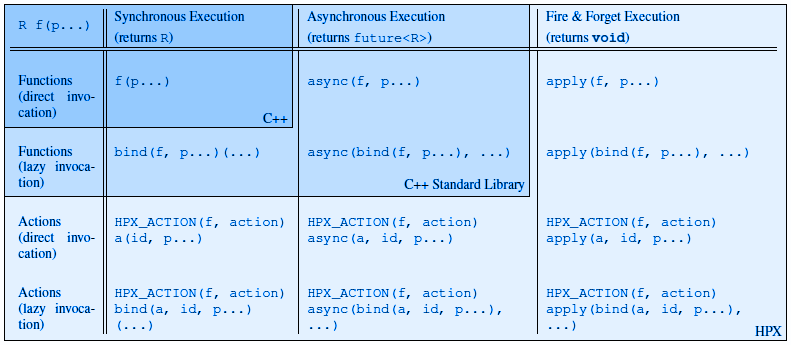
\includegraphics[scale=0.72]{images/hpx_the_api.png}
\caption[Overview of the main API exposed by HPX]{Overview of the main API exposed by HPX}
\label{fig:hpx-api}
\end{figure}

HPX provides several ways to apply an action. Its API exposes three different ways of executing a function, locally on the same physical locality as the invocation site or remotely on a different locality:

\begin{itemize}
\item ``\textbf{Synchronous function execution}\\
  This is the most natural way of invoking a C++ function. The caller ’waits’ for the function to return, possibly providing the result of the function execution. In HPX, synchronously executing an action suspends the current thread relinquishing the processing unit for other available work. Once the function is executed, the current thread is rescheduled.

\item \textbf{Asynchronous function execution}\\
  Asynchronous invocation of a function means that it will be scheduled as a new HPX thread (either locally or on another locality). The call to async will return almost immediately providing a new future instance which represents the result of the function execution. Asynchronous function execution is the fundamental way of orchestrating asynchronous parallelism in HPX.

\item \textbf{Fire \& Forget function execution}\\
  This is similar to asynchronous execution except that the caller has no means of synchronizing with the result of the operation. The call to apply schedules a local (or remote) HPX thread which runs to completion at its own pace. Any result returned from that function (or any exception thrown) is being ignored. This leads to less communication by not having to notify the caller.''\cite{kaiser2014hpx}
\end{itemize}


\begin{figure}[ht]
\centering
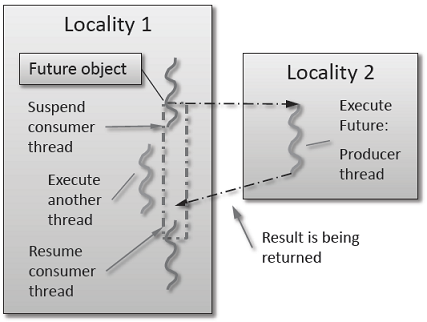
\includegraphics[scale=0.8]{images/future_schematics.png}
\caption[Schematic of a Future Execution]{Schematic of a Future Execution}
\label{fig:future_schematics}
\end{figure}

In C++, a future encapsulates a delayed computation. A future holds the result of an asynchronous call because the computation of the result has not completed yet~\cite{stroustrup2013c++}. HPX uses futures to synchronize the access to the value in a future by suspending any HPX threads requesting the result until the value is available. When a future is created, it spawns a new HPX thread which will execute the action associated with the future. The new thread is spawned either remotely with a parcel or locally by being placed into the thread queue.  Utilizing futuers allows HPX to schedule work early in a program so that when the function value is needed it will already be calculated and available (Figure \ref{fig:future_schematics})~\cite{kaiser2009parallex}.

\iffalse
\subsection{HPX Hello World Example}
Listing \ref{lst:hpx_hello_world}~\cite{hpx_hello} is a simple program that prints out a hello world message on every OS-thread on every locality.

\begin{lstlisting}[language=C, frame=single, numbers=left, basicstyle=\footnotesize, caption=HPX Hello World\label{lst:hpx_hello_world}]
int main() {
  std::vector<hpx::naming::id_type> localities =
  hpx::find_all_localities();
  std::vector<hpx::lcos::future<void> > futures;
  futures.reserve(localities.size());
  for (hpx::naming::id_type const& node : localities) {
    typedef hello_world_foreman_action action_type;
    futures.push_back(hpx::async<action_type>(node));
  }
  hpx::wait_all(futures);
  return 0;
}
\end{lstlisting}

Using the \verb|hpx::find_all_localities()| function, we get a list of all available localities and put them into a vector. Then, we reserve storage space for futures, one for each locality. Looping through all the localities, we asynchronously start a new task on each locality. The task is encapsulated in a future, which can be queried to determine if the task has completed. \verb|hpx::wait_all()| returns when all of the futures have finished.

Listing \ref{lst:hello_world_foreman} ~\cite{hpx_hello} illustrates the \verb|hello_world_foreman()| function which is used to make \verb|hello_world_foreman| action. \verb|hpx::get_os_thread_count()| returns the number of worker OS-threads in use by the current locality. \verb|hpx::find_here()| returns the global name of the current locality. Inside the for loop, we populate a set with the OS-thread numbers of all OS-threads on this locality. When the hello world is printed on a particular OS-thread, we remove it from the set. As long as there are elements in the set, we keep scheduling HPX-threads. Note that because HPX features work-stealing task schedulers, we have no way of enforcing which worker OS-thread will actually execute each HPX-thread. Inside the while loop, in each iteration we create a task for each element in the set of OS-threads that have not said ``Hello world''. Each of these tasks is encapsulated in a future. Eventually, we wait for all of the futures to finish. The \verb|hpx::lcos::wait_each| function takes two arguments: a binary callback, and a vector of futures. The callback takes two arguments; the first is the index of the future in the vector, and the second is the return value of the future. \verb|hpx::lcos::wait_each| doesn't return until all the futures in the vector have returned. The macro \verb|HPX_PLAIN_ACTION| defines the boilerplate code necessary for the function \verb|hello_world_foreman| to be invoked as an HPX action.

\begin{lstlisting}[language=C, frame=single, numbers=left, basicstyle=\footnotesize, caption=Hello World Foreman\label{lst:hello_world_foreman}]
void hello_world_foreman() {
  std::size_t const os_threads = hpx::get_os_thread_count();
  hpx::naming::id_type const here = hpx::find_here();
  std::set<std::size_t> attendance;
  for (std::size_t os_thread = 0; os_thread < os_threads; ++os_thread) {
    attendance.insert(os_thread);
  }
  while (!attendance.empty()) {
    std::vector<hpx::lcos::future<std::size_t> > futures;
    futures.reserve(attendance.size());
    for (std::size_t worker : attendance) {
      typedef hello_world_worker_action action_type;
      futures.push_back(hpx::async<action_type>(here, worker));
    }
    hpx::lcos::local::spinlock mtx;
    hpx::lcos::wait_each(
    hpx::util::unwrapped([&](std::size_t t) {
      if (std::size_t(-1) != t) {
        boost::lock_guard<hpx::lcos::local::spinlock> lk(mtx);
        attendance.erase(t);
      }
    }),
    futures);
  }
}
HPX_PLAIN_ACTION(hello_world_foreman, hello_world_foreman_action);
\end{lstlisting}


\fi
